%!TEX root = thesis.tex

\chapter{Evaluation}
\label{ch:Evaluation}
The implementation of the I-POMDP framework was evaluated by training a policy for the \emph{``Where's Waldo?''} game described in Chapter \ref{ch:IPOMDP} and comparing the performance of the resulting policy to the performance of a greedy policy, a random policy, and a policy that always focuses on the center of the image. 

The policies were trained on a $7 \times 7$ grid where the grid represents the image and each grid location represents a state and an action, i.e. a location where Waldo can be found in and a location the agent can fixate on. The number of actions available to the agent are therefore equal to the number of states, namely $49$.

Both observation models mentioned in Section \ref{sec:ObservationModelImpl} were used to train policies and the default values presented in Section \ref{sec:PolicyTraining} were used in both cases.

\section{Training a Policy Using the Exponential Model}
\label{sec:PolicyExp}
The policy parameters for the policy learned when training with the exponential model for observations can be seen in Figure \ref{fig:ExpPolicyTheta}. This policy favors fixating on locations where the agent's belief is strong, since the values on the diagonal of the policy parameter matrix\footnote{See Section \ref{sec:LogisticPolicies} for an explanation of the policy parameter matrix} are relatively large. An agent using this policy would therefore with a high probability fixate on locations where it beliefs the target is located -- in other words, act greedy.

On both sides of the diagonal we again notice large parameter values, but not as large as on the diagonal itself. This can be interpreted as the second best choice of fixation. Fixating on locations close to the location where the belief is highest will therefore occur with a high probability. This policy could therefore be interpreted as a greedy policy with a slight tendency for curiosity.

\begin{figure}[!htp]
  \centering
  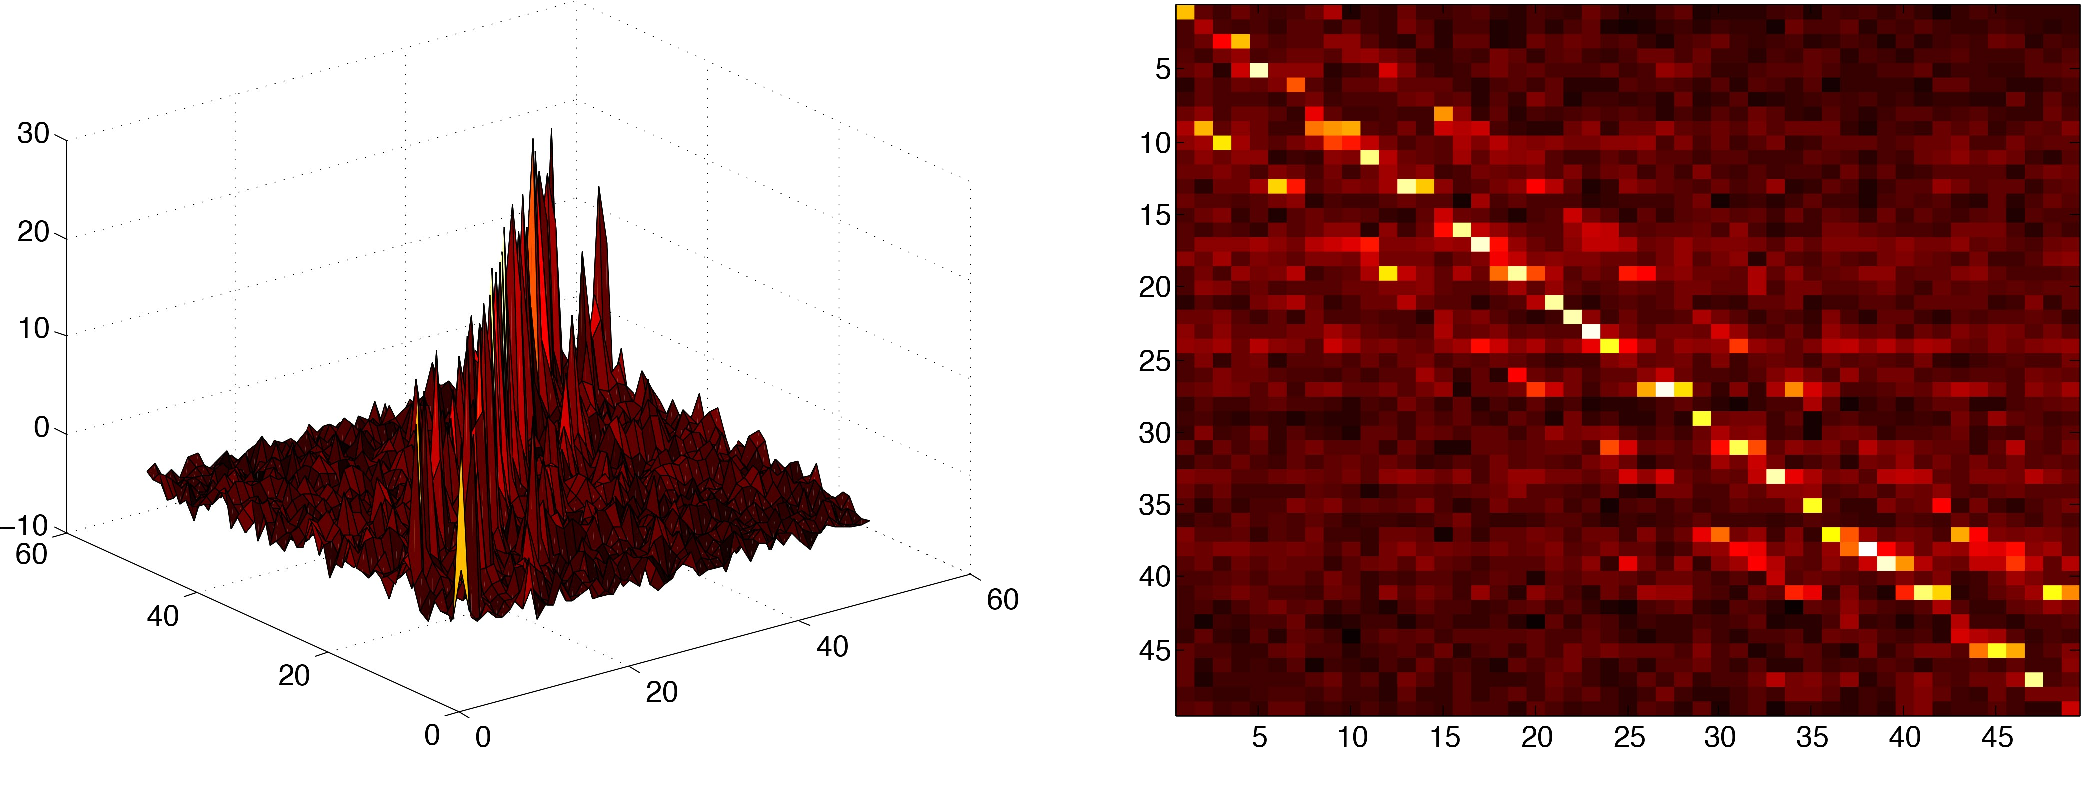
\includegraphics[width=1\textwidth]{figures/exp_policy_theta}
  \caption{The $49 \times 49$ policy parameter matrix $\theta$ trained using the exponential model for observations. \textbf{Left:} Relatively large values on the diagonal, slightly lower values on both sides of the diagonal. \textbf{Right:} The heat map shows clearly the two off-diagonal lines and the relatively large diagonal values.}
  \label{fig:ExpPolicyTheta}
\end{figure}
\FloatBarrier

\noindent
The learning curve for the policy can be seen in Figure \ref{fig:AverageRewardsExp}. It shows that the policy improves fast the first 200 training iterations, as the average rewards in each training iteration get higher and higher (less negative). The policy improvement continues slowly until after around 800 iterations where the learning converges.

\begin{figure}[!htp]
  \centering
  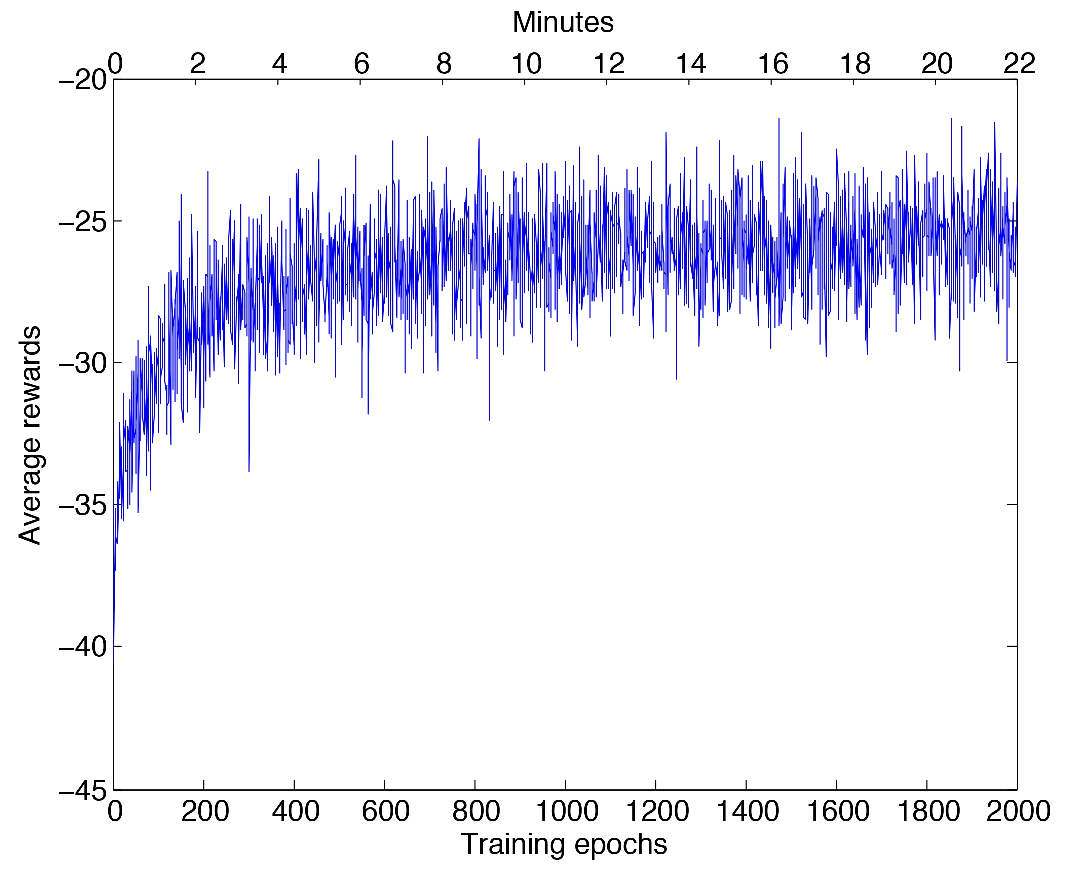
\includegraphics[width=0.5\textwidth]{figures/average_rewards_exp_2x}
  \caption{Average rewards per training iteration while training a policy using the exponential model for observations.}
  \label{fig:AverageRewardsExp}
\end{figure}

\section{Training a Policy Using the Human Eye Model}
The policy parameters for the policy learned when training with the human eye model for observations are very different from the parameters learned in Section \ref{sec:PolicyExp}. Instead of relatively large values on the diagonal, this policy's parameter matrix has less variance in the parameter values but a clear horizontal band of higher values across the middle of it. See Figure \ref{fig:EyePolicyTheta}.

\begin{figure}[!htp]
  \centering
  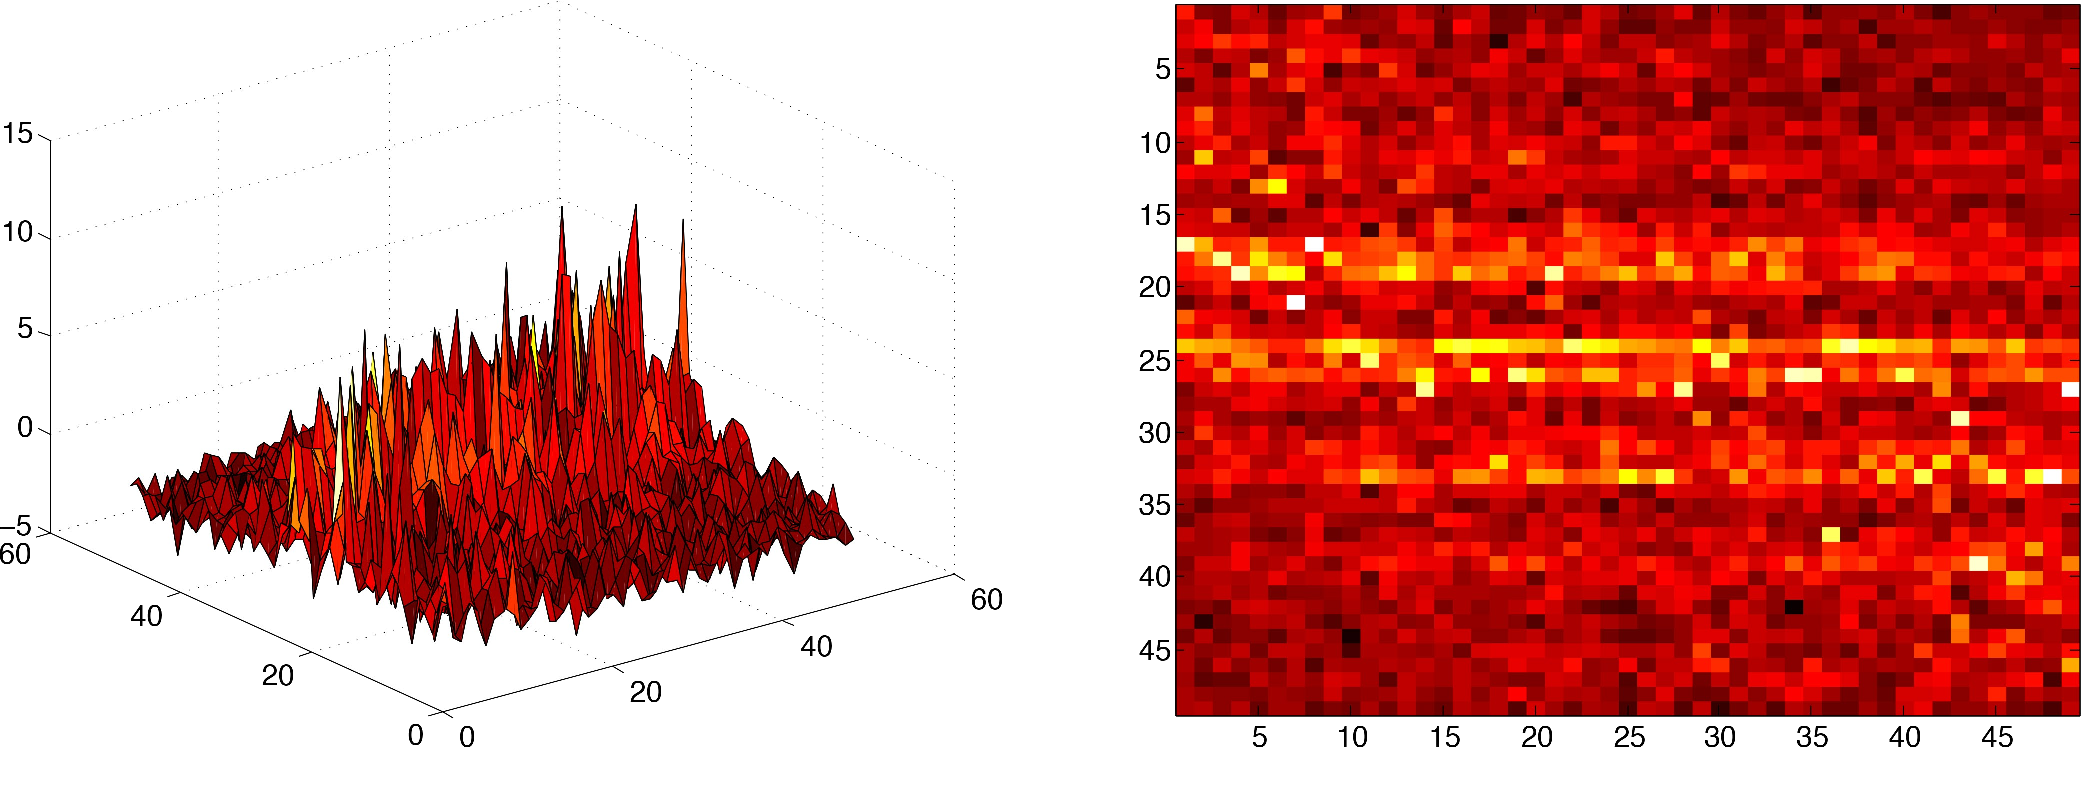
\includegraphics[width=1\textwidth]{figures/eye_policy_theta}
  \caption{The $49 \times 49$ policy parameter matrix $\theta$ trained using the human eye model for observations. \textbf{Left:} Relatively large values across the middle part of the parameter matrix and low values near the top and bottom. \textbf{Right:} Difference between the smallest and largest values not as evident as for the exponential model. Larger values across the center of the matrix.}
  \label{fig:EyePolicyTheta}
\end{figure}
\FloatBarrier

\noindent
To interpret this policy's parameter matrix we first note that on a $7 \times 7$ grid, location number $25$ would be in the center of the grid. With that in mind we can assume that this policy favors fixating on locations around the center of the image.

\begin{figure}[!htp]
  \centering
  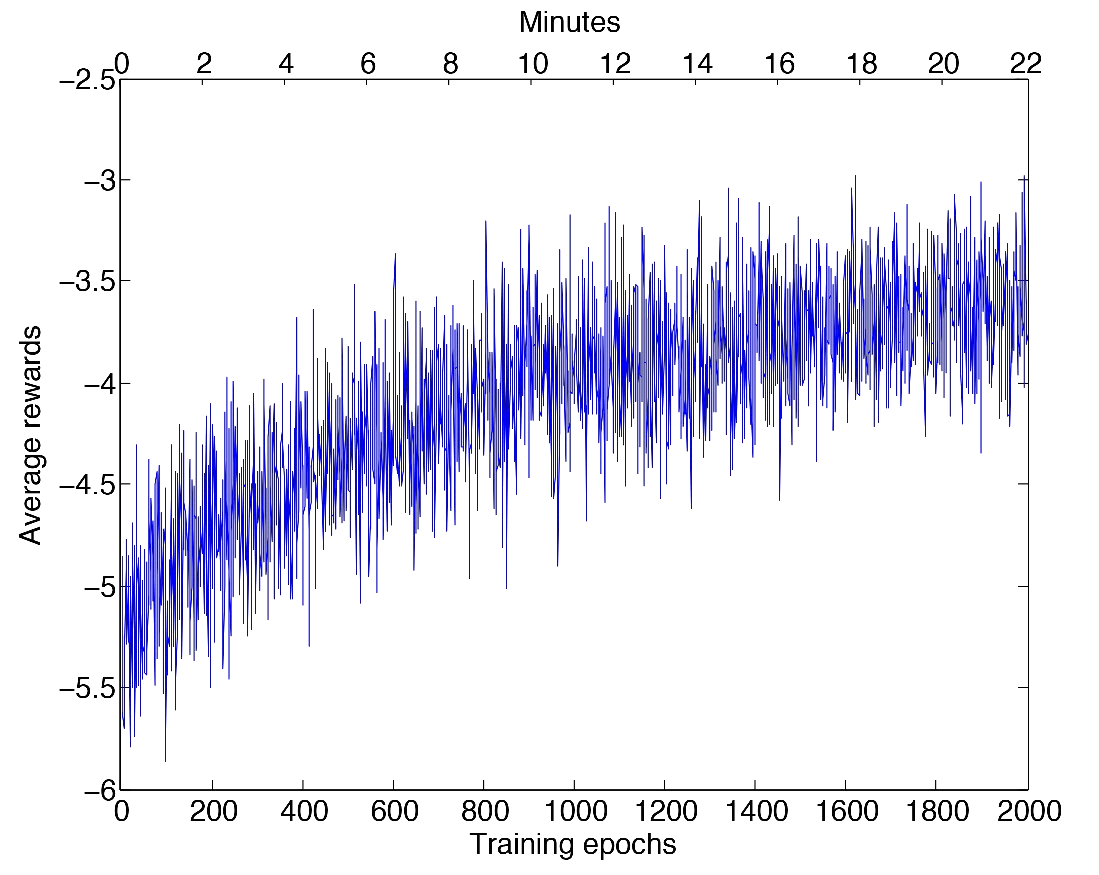
\includegraphics[width=0.5\textwidth]{figures/average_rewards_eye_2x}
  \caption{Average rewards per training iteration while training a policy using the human eye model for observations.}
  \label{fig:AverageRewardsEye}
\end{figure}

\noindent
The learning curve for the policy can be seen in Figure \ref{fig:AverageRewardsEye}. The first thing we notice is that the average rewards per training iteration are higher than during training of the policy in \ref{sec:PolicyExp}. This comes from the fact that the human eye model for observations has a wider field of view than the exponential model, which only sees a small part of the image very clearly.

The policy improves steadily for around 1600 iterations and after that the learning converges.

\section{Performance Comparison}
The performance of both learned policies was compared to the performance of a greedy policy, a random policy, and a policy that always focuses on the center of the image. The comparison was performed by simulating the search for ``Waldo'' with each policy $4,900$ times and recording each time how many fixations it took before the agent's highest belief matched the true location of ``Waldo''.

\subsection{Policy Using an Exponential Model}
All the policies perform similarly for the first 5 fixations, with the trained policy performing slightly better than the others, but after 6 fixations the random policy performs best. The exponential model for observations has a very narrow view and therefore does not fully exploit the potential of the I-POMDP algorithm. For each fixation the agent can only obtain reliable information about the image from the exact location it is fixating on, while the information in the surrounding locations is very noisy. This can make the agent's belief unreliable. As mentioned in Section \ref{sec:PolicyExp} this policy is very similar to the greedy policy and using a greedy policy when the belief is unreliable will result in poor performance. The trained policy is however a stochastic policy and therefore performs better than the greedy policy. The random policy benefits from the fact that it is not dependent on the noisy belief. It should also be noted that a policy that does not fixate on every location will eventually perform worse than random.

The comparison of the policies using the exponential model for observations can be seen in Figure \ref{fig:PolicyComparisonExp}.

\begin{figure}[!htp]
  \centering
  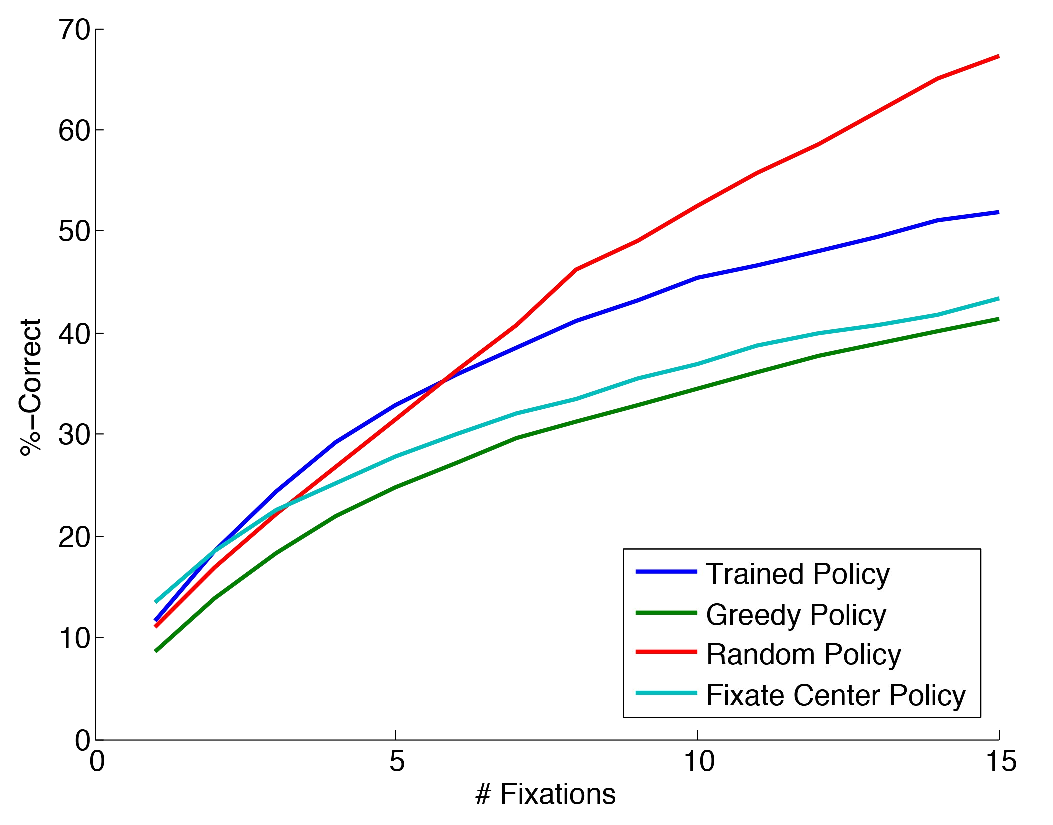
\includegraphics[width=0.5\textwidth]{figures/policy_comparison_exp2}
  \caption{Performance comparison of policies using the exponential model for observations.}
  \label{fig:PolicyComparisonExp}
\end{figure}

\subsection{Policy Using a Human Eye Model}
The human eye model for observations has a wider view than the exponential model and therefore the agent can not only obtain reliable information about the image from the location it fixates on, but also the locations surrounding it. This gives the trained policy an advantage because it exploits the potential of the I-POMDP algorithm. For this reason the trained policy outperforms the other policies as can be seen in Figure \ref{fig:PolicyComparisonEye}.

\begin{figure}[!htp]
  \centering
  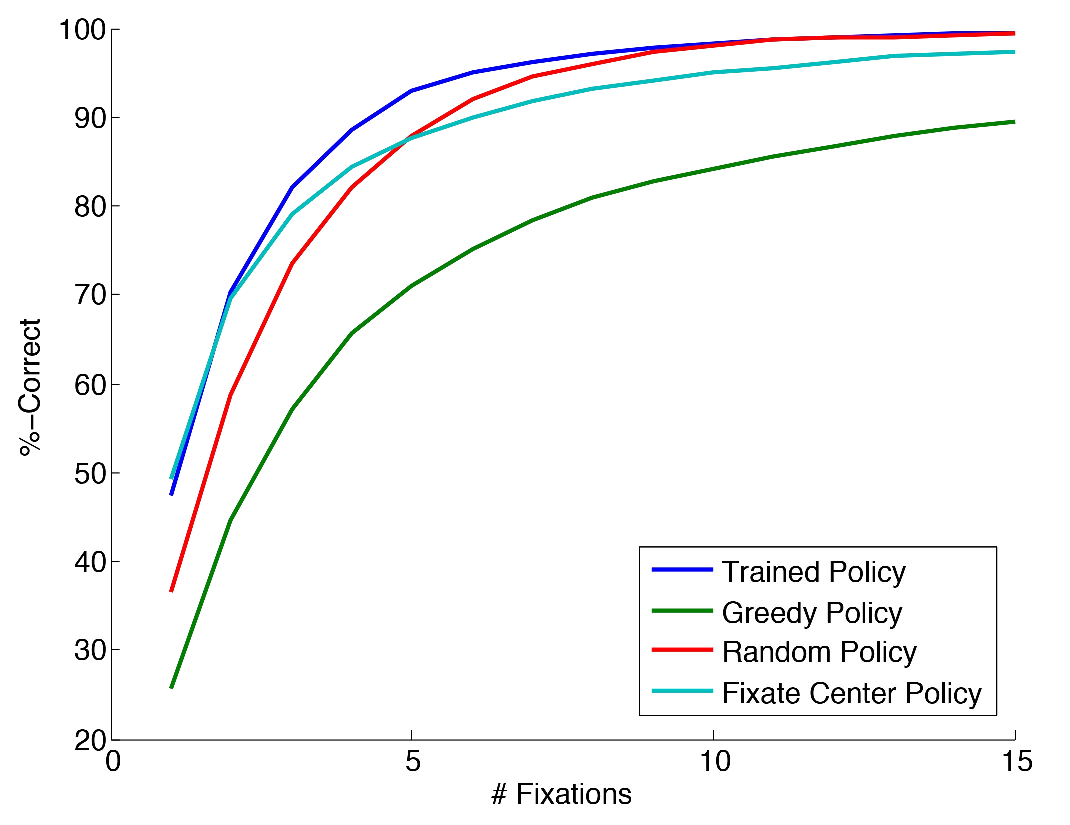
\includegraphics[width=0.5\textwidth]{figures/policy_comparison_eye2}
  \caption{Performance comparison of policies using the human eye model for observations.}
  \label{fig:PolicyComparisonEye}
\end{figure}

\noindent
The greedy policy proves to be a poor strategy in this case as well.
